	\section{Introduction}
	Ce document regroupe toutes les informations relatives à la gestion du projet et du processus de développement.Ce document est mis à jour régulièrement afin de permettre à tout moment d'avoir un aperçu de l'avancement du projet.
\section{Organisation}
	L'annexe A (/Documentation/Annexes/A) contient les directives qui ont été données au début de ce projet. Ces directives sont la ligne directrice concernant l'organisation du projet. 
	\subsection{Séances}
		Pour chaque séance, un procès verbal est rédigé par M. Elias Medawar.
	\begin{itemize}
		\item Des séances hebdomadaires seront effectuées avec M. Dany Mezher, le responsable externe .
		\item Une séance est tenue une semaine sur deux via Skype avec Mme Mugellini et M. Abou Khaled, les responsables internes.
		\item Au moins une séance est organisée avec les experts M. Roland Marro et M. Marc Wuergler via Skype.
	\end{itemize}
	\subsection{Site internet}
		Un site internet est mis en ligne et il est disponible à l'adresse suivante: \url{https://forge.tic.eia-fr.ch/projects/esibpad} \\
		Mme Mugellini et M. Abou Khaled peuvent utiliser leur login AII pour accéder aux données.\\
		Pour les autres personnes, des comptes ont été créés par le service informatique de l'école. Les comptes sont valides jusqu'au 31.12.2011. \\[1cm]
		
		
		\begin{table}[H]
			\centering
			\begin{tabular}{|c|c|}
				\hline M.Dany Mezher &  \\ 
				\hline   Username : &  dany.mezher   \\ 
				\hline   Password : & voir mail     \\ [0.2cm]
				\hline M.Marc Wuergler & \\ 
				\hline   Username : &  marc.wuergler  \\ 
				\hline   Password : & voir mail \\ [0.2cm]
				\hline M.Roland Marro &  \\ 
				\hline   Username :&  roland.marro  \\ 
				\hline   Password : & voir mail     \\
				\hline
			\end{tabular} 
			\caption{\label{tab.login}Données de login pour les personnes externe à l'EIA-FR}
		\end{table}
	
		Le site contiendra:
	 	\begin{itemize}
	 		\item le journal de bord :\url{https://forge.tic.eia-fr.ch/projects/esibpad/wiki}
			\item Les PVs :\url{https://forge.tic.eia-fr.ch/projects/esibpad/documents} 
			\item La documentation sous format PDF:\url{https://forge.tic.eia-fr.ch/projects/esibpad/documents} 
		\end{itemize}
	\subsection{Communication}
		Le moyen de communication principal est l'e-mail.\\
		\begin{table}[H]
			\begin{tabular}{|l|l|l|}
				\hline  Nom & email  & Téléphone [Fixe, Mobile]  \\ 
				\hline M. Würgler Marc & marc.wuergler@sunrise.ch  & +41 26 660 03 04, +41 78 609 49 44  \\ 
				\hline M. Marro Roland & marror@fr.ch  & +41 26 305 31 61  \\ 
				\hline M. Dany Mezher	& dany.mezher@fi.usj.edu.lb & +961 142 134 1,+961 700 100 30  \\ 
				\hline Mme Elena Mugellini & elena.mugellini@hefr.ch &  +41 26 429 68 70\\ 
				\hline M. Omar Abou Khaled & omar.aboukhaled@hefr.ch  &  +41 26 429 65 89\\ 
				\hline M. Elias Medawar & elias.medawar@edu.hefr.ch  &  +961 712 900 72, +41 764 090 330\\ 
				\hline 
			\end{tabular} 
			\caption{Résumé des adresses e-mail et des numéros de téléphones.}			
		\end{table}
	
		Des rendez-vous pour des vidéo-conférences seront organisés à l'aide de \gls{Skype}.
\section{Planification}
	\subsection{Plan global}
	 \EPSFIGTEXTWIDTH{../comon/figures/timeLineDetail.pdf}{Vue global du planning du projet avec les milestones}{planGlobDet}

	 \subsection{Description des jalons}

		 \begin{longtable}{|c|l|p{10cm}|}

		 \hline  \textbf{Nom} & \textbf{Date}  & \textbf{But à atteindre}  \\ 
		 \endfirsthead
		  \multicolumn{3}{|r|}{{suite de la page précédente}} \\ \hline
		\hline  \textbf{Nom} & \textbf{Date}  & \textbf{But à atteindre}  \\ 
		 \endhead
		  \multicolumn{3}{|r|}{{Suite à la page suivante}} \\ \hline
		 \endfoot
		 \endlastfoot
		 \hline  Milestone 1 & 03.06.11  & 
		 	\begin{itemize}
		 	 		\item Cahier des charges établi et validé.
		 			\item La première version du \gls{SPMP} est rédigée.
		 	\end{itemize}   \\ 
		 \hline  Milestone 2 & 10.06.11  & 
		 	\begin{itemize}
		 	 		\item Pouvoir déployer une simple application sur l'iPhone et l'iPad.
		 			\item Un environnement de développement local est mis en place, avec des Web Services de test ainsi que des données de test.
		 	\end{itemize}   \\ 
	 	 \hline  Release 0.1 & 17.06.11  & 
		 	\begin{itemize}
		 	 		\item La page d'accueil de l'application avec les différents menus est réalisée.
		 			\item La page de paramètre de l'application est réalisée.
		 	\end{itemize}   \\ 
	 	 \hline  Release 0.2 & 01.07.11  & 
		 	\begin{itemize}
		 	 		\item Afficher la carte du campus.
		 	 		\begin{enumerate}[a)]
	 	 				\item La position actuelle de l'utilisateur sera détectée à l'aide du \gls{GPS} de l'appareil et affichée sur la carte.
	 	 				\item L'utilisateur peut, à l'aide de la fonction <<chercher>> : trouver l'emplacement d'un cours, le bureau d'une personne ou le lieu d'un événement.
	 	 				\item Les informations de la carte sont enregistrées sur le serveur et peuvent être mises à jour à tout moment. Un système de cache évite de recharger la carte à chaque visite.
	 	 			\end{enumerate}
		 	\end{itemize}   \\ 
		 \hline  Release 0.3 & 13.07.11  & 
 		 	\begin{itemize}
 		 	 		\item Permettre aux professeurs et aux étudiants d'afficher leurs horaires.
	 		 	 	\begin{enumerate}[a)]
	 		 	 			\item Quand on clique sur un cours, l'emplacement de ce dernier est affiché sur la carte.
	 		 	 			\item L'utilisateur peut sauvegarder son horaire sur l'appareil pour un accès offline.
	 		 	 		\end{enumerate}
 		 	\end{itemize}   \\ 
		\hline  Release 0.4 & 22.07.11  & 
 		 	\begin{itemize}
 		 	 		\item Permettre de consulter les nouvelles du campus.
	 		 	 	\begin{enumerate}[a)]
	 		 	 			\item Si une nouvelle est liée à un lieu, permettre de l'afficher facilement sur la carte.
	 		 	 		\end{enumerate}
 		 	\end{itemize}   \\
		\hline  Release 0.5 & 03.08.11  & 
 		 	\begin{itemize}
 		 	 		\item Permettre l'accès à l'annuaire de l'université. 
	 		 	 	\begin{enumerate}[a)]
		 	 				\item Quand on clique sur un numéro de téléphone, l'appel est lancé.
		 	 				\item Quand on clique sur une adresse mail, la fenêtre d'envoi de mail de l'appareil est ouverte.
		 	 			\end{enumerate}
 		 	\end{itemize}   \\
	 	\hline  Release 0.6 Version 1 & 03.08.11  & 
 		 	\begin{itemize}
 		 	 		\item Permettre aux étudiants de consulter le résultat des examens. \textbf{Cet objectif est conditionné par l'accord de l'administration et du service informatique de l'\gls{ESIB}.}
 		 	\end{itemize}   \\  
	 	\hline  Milstone 3 &  19.08.11 &
	  		 	\begin{itemize}
	  		 	 		\item L'application est publiée sur l'App store.
	  		 	 		\item La documentation est finie.
	  		 	 		\item La présentation finale est prête.
	  		 	\end{itemize}   \\  
		 \hline 
		\caption{\label{tab.DescMils}Description des jalons. Les releases sont considérées comme des jalons.} \label{grid_mlmmh} \\
	 \end{longtable} 

	 \begin{landscape}
	 	 \subsection{Planification détaillé le 1 juin 2011}
		 \begin{figure}[H]
			 \begin{center}	
				 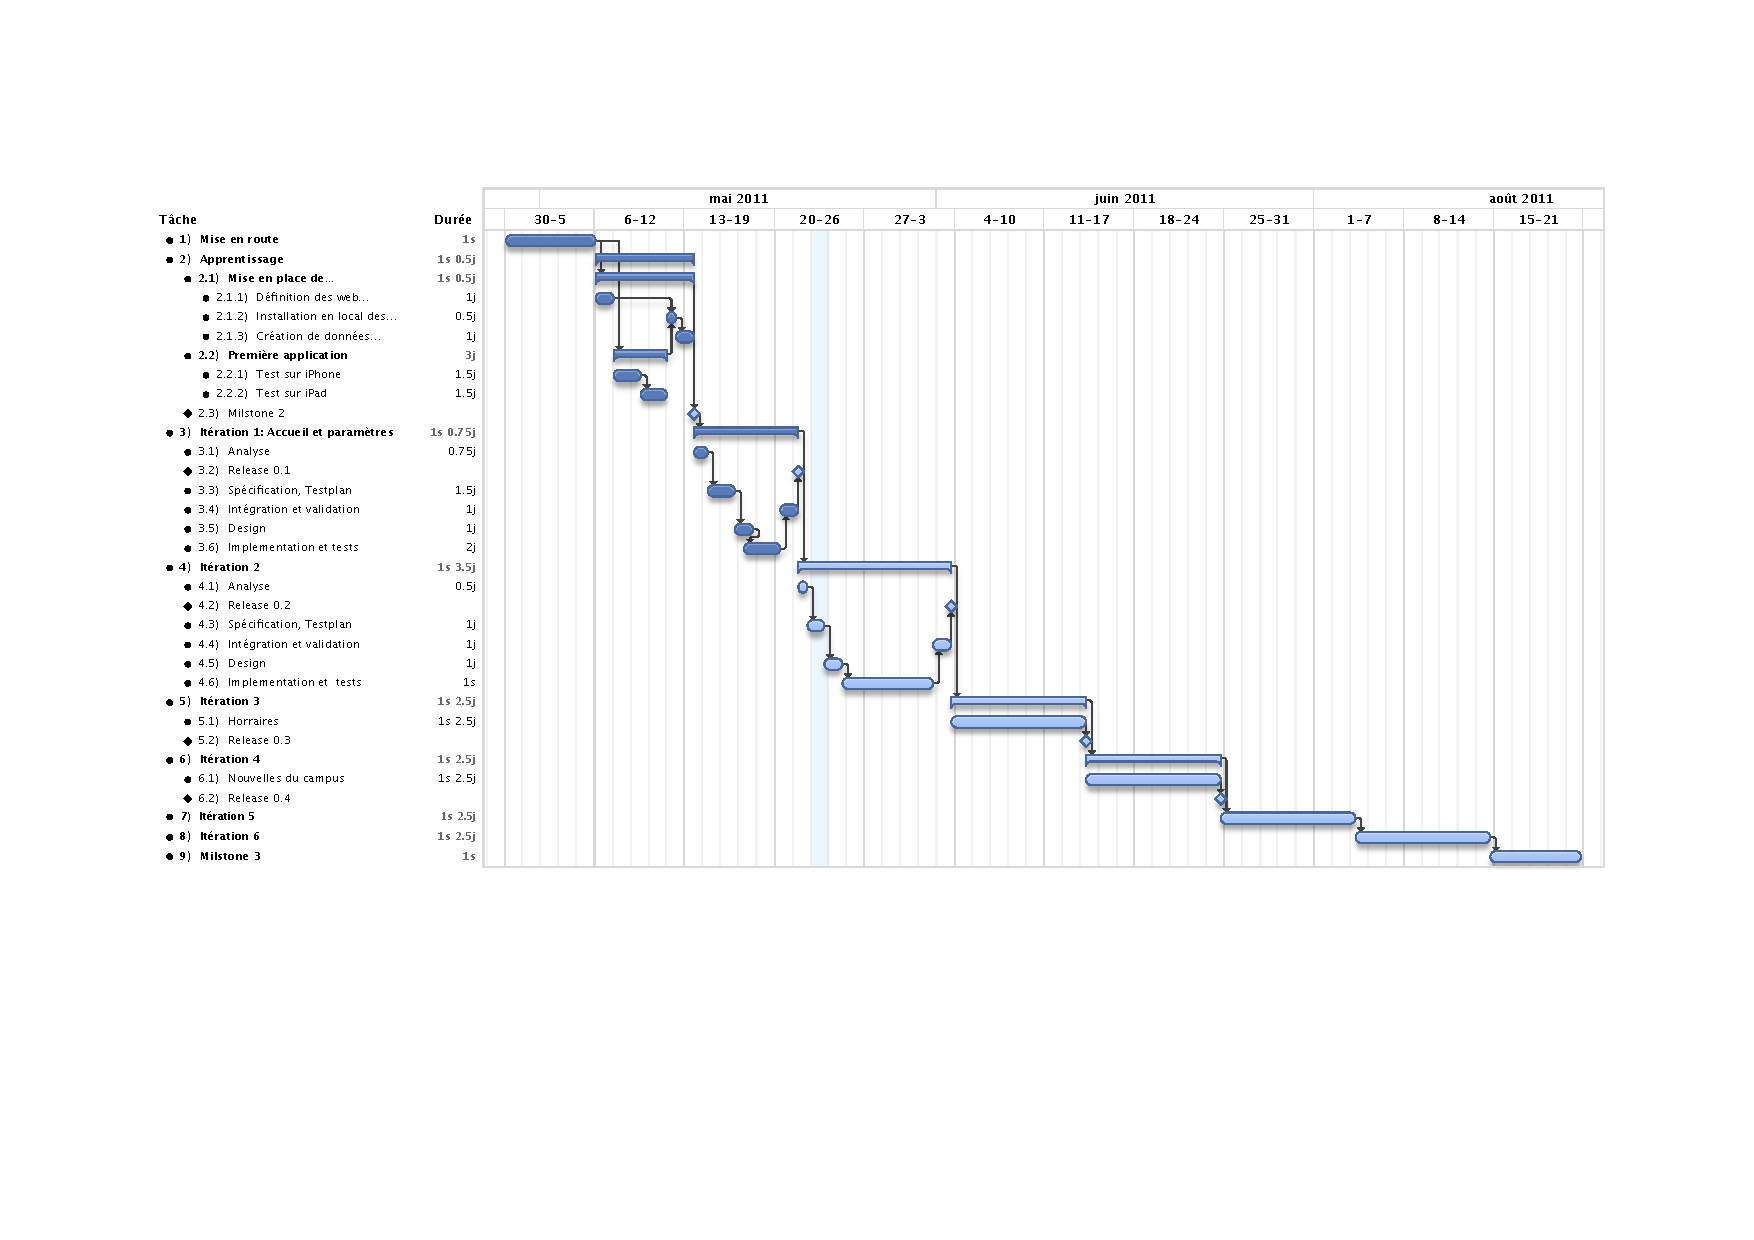
\includegraphics[height=0.8\textwidth]{../comon/figures/planningV2.pdf}
				 \end{center}			
				 \caption{Vue globale du planning du projet avec les milestones}			
				 \label{planV1}			
		 \end{figure}	
	 \end{landscape}
	 La planification détaillée de chaque itération n'est pas encore faite, elle sera faite au début de chaque itération et en prenant en considération l'expérience acquise lors des itération précédentes. 
\section{Processus technique}
Sur la Figure~\ref{planGlobDet} nous pouvons voir que nous allons travailler par itérations. Dans ce chapitre, voici une définition plus détaillée d'une itération 
	 \EPSFIGTEXTWIDTH{../comon/figures/vModel.pdf}{Illustration du modèle de développement en V qui est appliqué à chaque itération. }{vModel}
\textit{``Le modèle du cycle en V a été imaginé pour pallier le problème de réactivité du modèle en cascade. Ce modèle est une amélioration du modèle en cascade qui permet, en cas d'anomalie, de limiter un retour aux étapes précédentes. Les phases de la partie montante doivent renvoyer de l'information sur les phases en vis-à-vis lorsque des défauts sont détectés afin d'améliorer le logiciel.
De plus, le cycle en V met en évidence la nécessité d'anticiper et de préparer dans les étapes descendantes les « attendus » des futures étapes montantes : ainsi les attendus des tests de validation sont définis lors des spécifications, les attendus des tests unitaires sont définis lors de la conception, etc.
Le cycle en V est devenu un standard de l'industrie du développement de logiciel et de la gestion de projet depuis les années 1980. ``}\footnote{Définition selon Wikipedia: http://fr.wikipedia.org/wiki/Cycle\_de\_développement\_logiciel)\#Cycle\_en\_V}\\[1cm]

Ainsi cette approche sera répétée à chaque release pour arriver au but qui a été fixé.
\section{Gestion des risques}
Ce chapitre rassemble les divers risques qui mèneraient à un échec du projet. Le but est de mettre à jour les risques après chaque itération, et de faire qu'ils diminuent au plus vite. 
	\subsection{État le 01/06/2011  }
	\begin{table}[H]
	\begin{tabular}{|l|p{6cm}|l|l|l|p{6cm}|}
		\hline  Nr. & Risque & P  & DC & I & Mesure \\ 
		\hline  T1 & Le peu d'expérience dans le développement \gls{Objective-C} induit en erreur(sous estimation de la charge de travail, mauvaise architecture,etc) lors de la prise de décisions importantes au début du projet & 3 & 3 & 9 & Discuter les décisions avec des personnes ayant de l'expérience dans le domaine, prendre le temps d'apprendre les bases de l'\gls{Objective-C} au début du projet et prévoir une tâche simple pour la première itération.  \\ 
		\hline  T2 & Les Web Services ne sont pas encore opérationnels et peuvent retarder l'avancement du projet & 3 & 3 & 9 & Prévoir un environnement de développement en local avec des Web Services de test indépendants.  \\ 
		\hline  N1 & La méthodologie de travail au sein de l' \gls{EIA-FR} diffèrent trop de celle de l'\gls{ESIB}  et les méthodes ne conviennent pas à l'un ou l'autre parti.  & 1 & 2 & 2 & Organiser régulièrement des séances pour valider les décisions.  \\ 
		\hline  N2 & Sous-estimation de la charges de travail, dépassement du temps mis à disposition.  & 2 & 2 & 4 & Travailler par itération et se baser sur l'expérience acquise lors des itérations précédentes pour bien planifier les suivantes.Ne pas rester bloqué sur une étape sans demander de l'aide.  \\ 
		
		\hline 
	\end{tabular} 
	\caption{ Risques identifié au lancement du projet.\\ Légende :\\
Tx = Risque technique\\
Nx = Risque non technique\\
P = Probabilité  (1 peu probable / 3 très probable)\\ 
DC = Dégât et conséquence (1 peu / 3 grave)\\
I =  Importance ([1-2 petite][3-4 moyenne][5-9 sérieux])(P*DC)
}
	\end{table}
Les risques T1 et T2 qui sont d'une grande importance ont été pris en considération pour la planification.
	\subsection{État le 22/06/2011  }
	\begin{table}[H]
	\begin{tabular}{|l|p{6cm}|l|l|l|p{6cm}|}
		\hline  Nr. & Risque & P  & DC & I & Mesure \\ 
		\hline  {\color{green}T1} & Le peu d'expérience dans le développement \gls{Objective-C} induit en erreur(sous estimation de la charge de travail, mauvaise architecture,etc) lors de la prise de décisions importantes au début du projet & 2 & 3 & 6 & Ce risque à diminuer suite à l'expérience acquise durant la première itération.  \\ 
		\hline  {\color{green}T2} & Les Web Services ne sont pas encore opérationnels et peuvent retarder l'avancement du projet & 1 & 3 & 3 & Diminution suite à la création d'un environnement de test stable et contrôlable. Une première version des web services a été mis en place par le service informatique de l'\gls{USJ}  .  \\ 
		\hline  N1 & La méthodologie de travail au sein de l' \gls{EIA-FR} diffèrent trop de celle de l'\gls{ESIB}  et les méthodes ne conviennent pas à l'un ou l'autre parti.  & 1 & 2 & 2 & Organiser régulièrement des séances pour valider les décisions.  \\ 
		\hline  {\color{red}N2} & Sous-estimation de la charges de travail, dépassement du temps mis à disposition.  & 3 & 2 & 6 & Suite au retard pris lors de la première itération ce risque augmente.  \\ 
		
		\hline 
	\end{tabular} 
	\caption{ Risques après la première itération.\\ Légende :\\
Tx = Risque technique\\
Nx = Risque non technique\\
P = Probabilité  (1 peu probable / 3 très probable)\\ 
DC = Dégât et conséquence (1 peu / 3 grave)\\
I =  Importance ([1-2 petite][3-4 moyenne][5-9 sérieux])(P*DC)
}
	\end{table}
Les probabilité des risques T1 et T2  ont diminuer après la première itération tandis que celle du risque N1 a augmenté. On peut constater que globalement les risque diminue. Il faut travailler sur la planification pour diminuer au plus vite le risque N1.

\section{Gestion des configurations}
Afin de garder des traces de l'évolution du projet, des versions des sources des documents seront sauvegardées sur un serveur \gls{SVN}. La version courante du projet est hébergée à l'adresse suivante: \url{http://esibpad.googlecode.com/svn/trunk/}. Les releases seront stockés  à l'emplacement suivant:\url{http://esibpad.googlecode.com/svn/tags/} 

	 \EPSFIGTEXTWIDTH{../comon/figures/config.pdf}{Configuration pour la release 0.1. Les liens en rouges représentent la compatibilité entre composants.}{configExemp}


\section{Gestion de la documentation}
 La documentation sera conçue selon les différentes normes IEEE sur la documentation de software. Elle contiendra notamment les documents suivants:

\begin{enumerate}
	\item \gls{SPMP} - Software Project Management Plan (IEEE 1058).  Ce document contient toutes les informations concernant l'organisation d'un projet de développement de software . Il a pour but de rendre transparente l'organisation du projet et aide les chefs de projets à avoir un aperçu global de l'état d'avancement.
	\item \gls{SRS} - Software Requirements Specification(IEEE 830). Ce document contient la documentation concernant la spécification et l'analyse.
	\item \gls{SDD} - Software Design Description(IEEE 1016). Ce document contient la documentation concernant la conception  et l'implémentation.
	\item \gls{STD} - Software Test Documentation(IEEE 1016). Ce document contient la documentation concernant les tests effectués.
\end{enumerate}	

Il est important d'indiquer que la documentation ne sera pas complètement conforme à la norme, car cela représenterait une trop grande charge de travail. En effet, les différentes normes sont très complètes et plusieurs chapitres ne sont pas adaptés à notre projet. La variante de documentation qu'on utilise est inspirée de celle utilisé par la ``Hochschule Luzern `` (école d'ingénieurs Suisse alémanique dans laquelle j'ai eu l'occasion d'étudier durant 6 mois).

\section{Gestion des finances}
Ce travail fait partie du processus de formation et ne traite pas en détail de l'aspect financier.
\subsection{Ressources humaines}
\begin{itemize}
	\item 1 futur ingénieur HES  à 100\%  soit 40 heures par semaine durant 12 semaines. Une bourse est versée par  l'\gls{EIA-FR} à l'étudiant pour le transport jusqu'au Liban ainsi que le logement sur place. 
\end{itemize}
\subsection{Ressources matérielles}
\begin{itemize}
	\item 1 iPad2 et 1 iPhone 4  mis à disposition par l'\gls{EIA-FR}
	\item local de travail mis à disposition par l'\gls{ESIB}
\end{itemize}